% Jigsaw: PVLDB Vol. 20 / VLDB 2027 research-track submission.
% Official template: github.com/vldbproceedings/VLDB-Template (acmart.cls v2.19 + pvldb.sty).
% Format: two-column, 12 pages INCLUDING appendices (references excluded), SINGLE-BLIND
% (author names required on p1).

\documentclass[sigconf, nonacm]{acmart}

%%% do not modify the following VLDB block %%
%%% VLDB block start %%%
\usepackage{pvldb}
%%% VLDB block end %%%

%% Per-paper VLDB fields (placeholders until camera-ready).
\renewcommand\vldbdoi{XX.XX/XXX.XX}
\renewcommand\vldbpages{XXX-XXX}
\renewcommand\vldbavailabilityurl{https://github.com/DoggoWoofWoof/Jigsaw}

%% Packages/macros used by the body beyond acmart defaults.
%% (acmart already provides booktabs, graphicx, amsmath/amssymb, and the
%%  proposition theorem environment -- do not redeclare those.)
\usepackage[most]{tcolorbox}
\usepackage{multirow}
\usepackage{algorithm}
\usepackage{algpseudocode}
\newtcolorbox{guaranteebox}[1][What Jigsaw guarantees]{colback=black!3,colframe=black!60,
  boxrule=0.5pt,left=6pt,right=6pt,top=5pt,bottom=5pt,arc=2pt,
  fonttitle=\bfseries,title={#1}}

\begin{document}

\title{Jigsaw: Memory-Bounded Exact Subgraph Matching on Million-Node Attributed Graphs}

\author{Swastik Mohapatra}
\affiliation{%
  \institution{PES University}
  \city{Bengaluru}
  \country{India}
}
\email{swastik9895@gmail.com}

\begin{abstract}
Exact subgraph matching enumerates every embedding of a small attributed query graph in a large data graph, and it underpins graph databases, knowledge-graph search, and program analysis. Exact solvers are memory-bound: run over the whole graph, the Glasgow Subgraph Solver enumerates all 15 test queries on CoraFull (19.8K nodes) but none once the graph reaches OGBN-Arxiv scale (169K nodes), and at a million nodes holding the graph together with the solver's candidate domains resident becomes impractical. We present \textbf{Jigsaw}, a retrieval-constrained matcher that keeps exact matching feasible under a fixed memory budget. Jigsaw partitions the data graph offline, retrieves a small set of candidate partitions per query with a coverage-trained encoder, expands them by one-hop boundary overlap, prunes by typed signature and exact label, and invokes the exact solver only inside the retrieved candidate. The guarantee is precise: every returned mapping is an exact match within the retrieved candidate under a configured discrete label semantics, verified by the solver alone, and the memory budget $K$ trades recall for footprint but never soundness; a bounded no-match result is not a certificate of global non-existence. On OGBN-MAG (1.9M nodes) Jigsaw solves \textbf{88.6\%} of 1{,}800 planted positives while a two-pass streaming implementation holds \textbf{2.4}\,GB instead of \textbf{10.2}\,GB for whole-graph residence ($4.2\times$ less). Because the value of learning depends on label selectivity, Jigsaw routes retrieval by an offline selectivity statistic: a classical label index dominates when labels are near-unique (96.7\% on MAG) and the coverage-trained encoder dominates under realistic class labels. We report both rather than a single winner, turning retrieval into a practical execution layer for exact verification rather than a neural replacement for it.
\end{abstract}

\keywords{exact subgraph matching, subgraph isomorphism, attributed graphs, graph retrieval, memory-bounded query processing, graph partitioning, learned retrieval}

\ccsdesc[500]{Information systems~Graph-based database models}
\ccsdesc[300]{Mathematics of computing~Graph algorithms}
\ccsdesc[300]{Computing methodologies~Machine learning approaches}

\maketitle

%%% do not modify the following VLDB block %%
%%% VLDB block start %%%
\vldbtopmatter
%%% VLDB block end %%%

\section{Introduction}

Subgraph isomorphism is a basic tool for motif discovery, scientific graph analysis, fraud search, and security auditing. The exact decision problem is NP-complete~\cite{ref_garey}; modern constraint solvers such as Glasgow~\cite{ref_glasgow} are strong, but large candidate domains and whole-graph residence still make them difficult to serve at scale. Learned retrieval can identify promising graph regions, but it cannot certify a match. Our question is whether retrieval can reduce the target enough for exact verification to fit a practical memory budget. Jigsaw uses the neural model only to choose where to search and leaves acceptance to Glasgow.

We call this design \emph{retrieval-constrained verification}. Jigsaw partitions a large graph, embeds queries and partitions in a shared space, retrieves a bounded set of partitions, stitches their overlap neighborhoods, prunes by typed structural signatures and exact labels, and then calls the verifier. If the candidate contains a valid embedding, Glasgow can certify it exactly. Missing a required region limits global completeness but cannot create a false match. FullCov trains the retriever against that specific failure event by requiring coverage of every partition touched by the planted match.

We evaluate the full path across CoraFull, OGBN-Arxiv, and MAG using two locked seeds, three sizes, six positive and two negative families, and six retrieval policies. At matched half-partition budgets the full cascade solves $94.2/92.8/88.6\%$ of planted positives on CoraFull/Arxiv/MAG (Table~\ref{tab:production_matrix}). Two operators put it there: coverage-aware training improves the fixed-budget retrieval operating points (Table~\ref{tab:loss_ablation}), and one-hop boundary overlap is the load-bearing recall step (Table~\ref{tab:design_ablation}). Examining every partition reaches $100\%$ on CoraFull/Arxiv but is a recall ceiling, not a scalable policy.

\paragraph{Contributions.}
\begin{itemize}
    \item We turn exact matching into a \textbf{memory-bounded service}: partition-wise streaming verifies OGBN-MAG (1.9M nodes) within a $2.4$\,GB budget versus $10.2$\,GB for whole-graph residence ($4.2\times$ less) and exposes a tunable memory--latency frontier that resident and prior learned-exact matchers do not. Under this budget, retrieval-constrained verification recovers $88.6\%$ of the $1{,}800$ planted MAG positives, where a direct whole-graph Glasgow call solves $0/15$ of the K-hop timeout control (Table~\ref{tab:scaling_latency}); the same substitution turns Arxiv's direct $0/15$ into $15/15$.
    \item We formulate the pipeline as coverage-conditioned exact verification, separating verifier soundness under the configured label semantics (always guaranteed) from retrieval completeness (a tunable budget knob), and prove the pruning stage is coverage-lossless.
    \item We introduce \textbf{FullCov}, which targets the weakest required partitions: Conditional Value-at-Risk (CVaR) averages the largest tail of their losses, and a top-$K$ barrier penalizes those below the retrieval cutoff.
    \item We provide a two-seed, three-dataset benchmark with positive and negative query families, exact-verification metrics, and an audited evaluation, measuring each candidate-shrinkage stage to show that boundary overlap is essential for recall while query-derived pruning preserves every covered match.
\end{itemize}

\section{Problem and Guarantee}
\label{sec:problem}

Let $G=(V,E,X)$ be a large attributed data graph and $Q=(V_Q,E_Q,X_Q)$ a query graph. The exact task asks for embeddings of $Q$ into $G$ that preserve edges, node types, and a discrete vertex-label map $\sigma$ under the solver's configured semantics. Whole-graph exact search is memory-bound: the verifier must hold $G$ and its candidate domains resident, which becomes infeasible as $G$ reaches millions of nodes (Section~\ref{sec:results}). Jigsaw instead constructs a candidate subgraph $G_C\subseteq G$ and runs the exact verifier only on $G_C$. Three claims are commonly conflated; we state precisely which ones Jigsaw guarantees.

\begin{guaranteebox}[What Jigsaw guarantees]
Fix a data graph $G$, query $Q$, label semantics $\sigma$, and memory budget $K$; Jigsaw returns a set $M$ of embeddings of $Q$ into $G$.
\textbf{(i)~Soundness.} Every $m\in M$ is an exact embedding under $\sigma$, certified by the Glasgow verifier on $G_C$ alone; no learned component can accept a match. The default $\sigma$ is an attribute hash, so acceptance is exact \emph{under $\sigma$} by construction; raw-attribute exactness is stronger, holds empirically on this benchmark (audited below), and is guaranteed by construction only with the optional raw-equality guard enabled.
\textbf{(ii)~Candidate-local completeness.} $M$ contains every embedding whose image lies inside the retrieved candidate $G_C$; matching-invariant pruning removes no valid embedding (Proposition~\ref{prop:lossless}).
\textbf{(iii)~Budget monotonicity.} Enlarging $K$ can only grow $G_C$, hence $M$, and never admits a spurious match; at $K=|\mathcal{P}|$ every partition is admitted and the run is complete under $\sigma$ whenever the verifier finishes.
Jigsaw does \emph{not} certify global non-existence: an empty $M$ means ``no match inside $G_C$,'' not ``no match in $G$.'' Recall of true matches is an empirical quantity we measure, not a worst-case bound.
\end{guaranteebox}

\paragraph{Coverage metric.}
Retrieval quality is governed by whether the candidate covers the match. Let $\mathcal{T}(Q)$ be the coarse partitions touched by a planted embedding and $R_K(Q)$ the retrieved top-$K$ partition set. We define
\begin{equation}
\mathrm{FullCov@K}(Q)=\mathbf{1}\left[\mathcal{T}(Q)\subseteq R_K(Q)\right].
\end{equation}
Partition recall@$K$ is $|\mathcal{T}(Q)\cap R_K(Q)|/|\mathcal{T}(Q)|$; FullCov@$K$ equals one only when recall is complete. One-hop boundary overlap expands $R_K$ before pruning, so FullCov is sufficient but not necessary: overlap can recover a required boundary node even when its home partition is not in the top $K$.

\paragraph{Budget as a soundness-preserving completeness dial.}
Soundness never depends on $K$: any returned match is a true match at every budget, so $K$ is a pure completeness control. At $K=|\mathcal{P}|$ (FilterAll) retrieval covers the whole partition set and matching-invariant pruning preserves every valid embedding, so the run is complete under $\sigma$ whenever the verifier finishes. As $K$ shrinks, the solved-by-budget curves of Section~\ref{sec:results} measure realized completeness under the timeout. A caller needing certainty pays for all partitions and sufficient verifier time; one needing speed accepts a quantified miss/timeout rate.

\paragraph{Label semantics and why acceptance is exact.}
The verifier consumes discrete labels $\sigma(v)$; by default we set $\sigma(v)=\mathrm{md5}(x_v)\bmod 10^{6}$, a hash of the full node attributes. Discretization is used only to shrink the retrieval and pruning domain, and because pruning is matching-invariant (Proposition~\ref{prop:lossless}) a hash collision can only enlarge the candidate the verifier inspects, never remove a valid embedding. Two exactness notions must be separated. Under $\sigma$-semantics the Glasgow certificate is exact by definition. Raw-attribute exactness is stronger, and the modular hash \emph{does} collide: across MAG's $742{,}524$ distinct node representations, $\mathrm{md5}\bmod 10^{6}$ yields only $524{,}328$ distinct codes, so $52.3\%$ of representations share a bucket and $34.4\%$ of nodes fall in a colliding bucket. A $\sigma$-certified mapping onto a collided node would be $\sigma$-exact but not necessarily raw-exact. We address this in two ways: (a) we audit every accepted mapping ($1{,}595$ solved positives, $87{,}536$ mapped node pairs) and find zero raw-attribute mismatches on this benchmark---an empirical result on the tested queries, not a worst-case bound; and (b) a drop-in raw-attribute equality guard on each returned mapping restores raw-exactness by construction for any $\sigma$. (Separately, a dataset-integrity check confirms all $1{,}800$ planted witnesses, $101{,}951$ pairs.) Section~\ref{sec:results} additionally reports a coarser $39$-class label regime, which stresses selectivity and motivates the retriever portfolio.

\section{Jigsaw Method}
\label{sec:method}

\begin{figure*}[t]
\centering
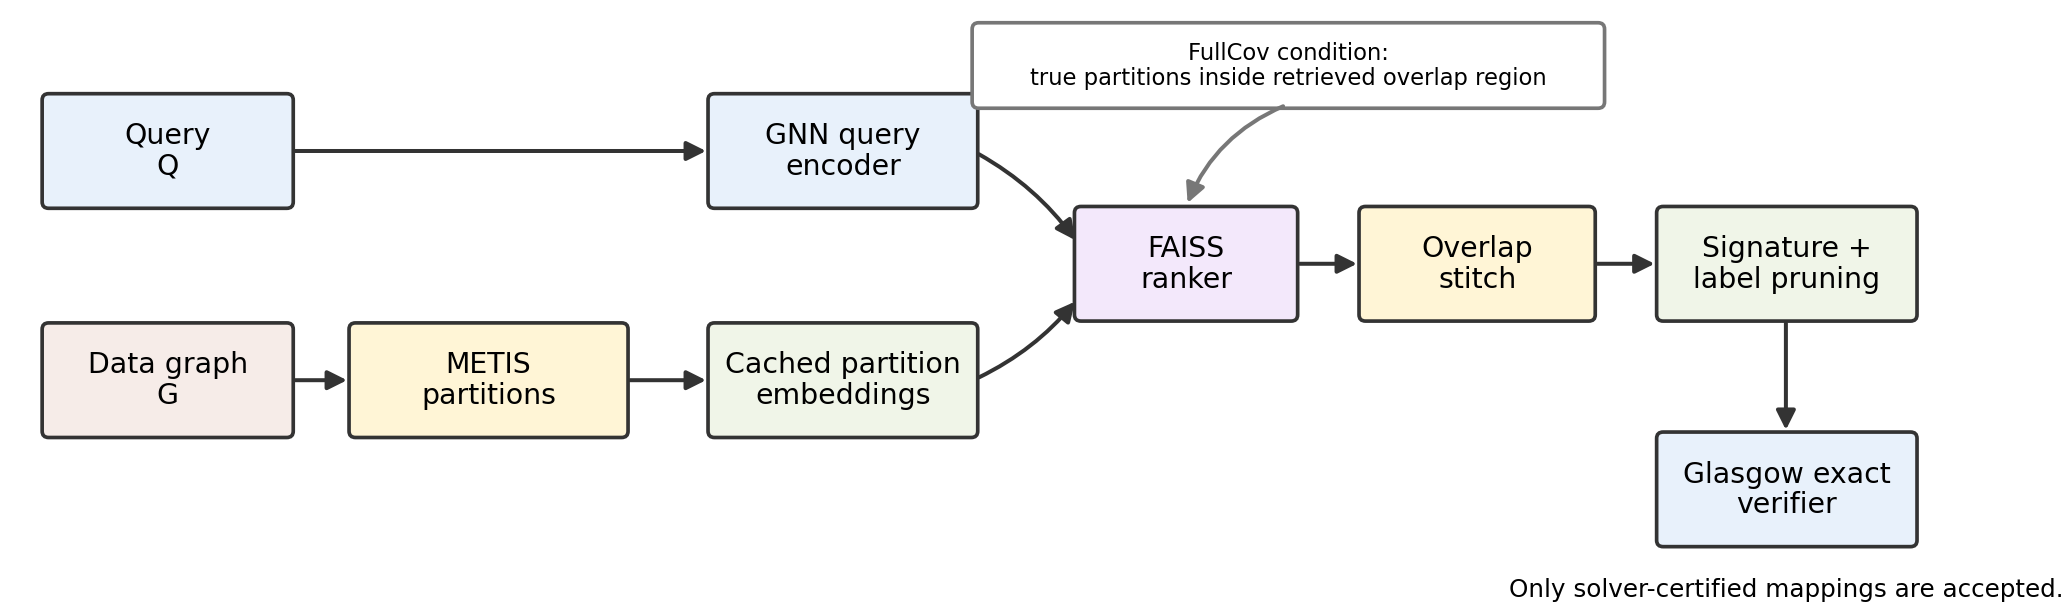
\includegraphics[width=0.86\textwidth]{fig_jigsaw_pipeline.png}
\caption{\textbf{Jigsaw pipeline.} Offline work partitions and embeds the target; online work embeds a query, retrieves coarse partitions, adds one-hop boundary overlap, prunes with query-derived invariants, and invokes Glasgow. The learned component ranks regions, but only Glasgow accepts a match. FullCov is the condition under which the candidate contains every partition the planted match needs.}
\label{fig:pipeline}
\end{figure*}

Figure~\ref{fig:pipeline} gives the dataflow. Offline, METIS partitions $G$ into fine and coarse blocks; the shared encoder embeds every coarse block once and FAISS indexes the normalized vectors. Online, Jigsaw embeds the query, retrieves coarse blocks, stitches boundaries, prunes, and verifies (Algorithm~\ref{alg:serving}).

\paragraph{Hierarchical localization and overlap cascade.}
Fine blocks give local structure; coarse blocks are the retrieval units. For each query Jigsaw computes $z_Q=f_\theta(Q)$ and ranks all coarse partitions by cosine similarity to the cached partition embeddings, retrieving the top $K$. True query neighborhoods often cross hard partition boundaries, so Jigsaw stitches each retrieved partition with its one-hop boundary nodes from adjacent partitions -- not the adjacent partitions in full -- raising recall before verification while still avoiding whole-graph search.

\paragraph{Pruning and verification.}
The stitched region is filtered by typed attribute signatures (node type plus hashed feature fingerprints) and exact labels before Glasgow verification; connected components become independent verifier calls. Both token sets are derived exclusively from the submitted query payload -- planted target-node IDs are evaluation metadata and never enter candidate construction or serving-time pruning. Only the exact verifier returns a match. As a running example, suppose a planted query touches blocks $p_4$ and $p_7$: if both rank in the top $K$, FullCov holds; if only $p_4$ ranks but the required nodes of $p_7$ lie on its boundary, overlap still completes the candidate; if an interior node of $p_7$ is never admitted, the bounded run may miss the match but cannot return an invalid one.

\begin{algorithm}[t]
\caption{Jigsaw online serving (one query)}
\label{alg:serving}
\begin{algorithmic}[1]
\Require target $G$ partitioned into coarse blocks $\mathcal{P}$ with cached embeddings $\{p_j\}$ and FAISS index; encoder $f_\theta$; query $Q$; budget $K$; label map $\sigma$
\Ensure set $M$ of exact embeddings of $Q$ inside the retrieved candidate
\State $z_Q \gets f_\theta(Q)$ \Comment{embed query}
\State $R \gets \textsc{TopK}(\mathrm{cos}(z_Q,\{p_j\}),\,K)$ \Comment{retrieve coarse blocks}
\State $G_C \gets \bigcup_{p\in R} p \,\cup\, \textsc{OneHopBoundary}(R)$ \Comment{stitch boundary overlap}
\State $G_C' \gets \{\,v\in G_C : \sigma(v)\in\sigma(V_Q)\ \wedge\ \mathrm{sig}(v)\in\mathrm{sig}(V_Q)\,\}$ \Comment{lossless prune (Prop.~\ref{prop:lossless})}
\State $M \gets \emptyset$
\For{each connected component $C$ of $G_C'$}
  \State $M \gets M \cup \textsc{Glasgow}(Q,C)$ \Comment{exact verify; sole accepting step}
\EndFor
\State \Return $M$
\end{algorithmic}
\end{algorithm}

\paragraph{FullCov objective.}
Standard contrastive training~\cite{ref_cpc} rewards high average similarity to positives, which can still leave one required partition ranked too low; Jigsaw optimizes the bottleneck. For query $i$, let $P_i$ be its required partitions and $u_{ij}=z_i^\top p_j/\tau_{\mathrm{cov}}$ the temperature-scaled similarity to partition $j$ ($\tau_{\mathrm{cov}}$ a fixed temperature). Each positive $j\in P_i$ receives
\begin{equation}
\begin{aligned}
c_{ij}&=-\log\frac{e^{u_{ij}}}{\sum_m e^{u_{im}}},\qquad
h_i=\max_{n\notin P_i}u_{in},\\[2pt]
\ell_{ij}&=c_{ij}+0.25\,\mathrm{softplus}(h_i-u_{ij}).
\end{aligned}
\end{equation}
For tail fraction $\rho$, $\mathrm{CVaR}_{\rho}$~\cite{ref_cvar} averages the largest $\lceil \rho|P_i|\rceil$ losses, so easy positives cannot hide the weakest one; a top-$K$ barrier $b_{ij}=\mathrm{softplus}(t_i(K)-u_{ij})$ pushes borderline positives above the cutoff $t_i(K)$, defined as the similarity of the $K$-th ranked partition for query $i$ (the retrieval boundary a positive must clear). The coverage loss is
\begin{equation}
\mathcal{L}_{\mathrm{cov}}=\mathrm{CVaR}_{\rho}(\{\ell_{ij}\})+0.35\,\mathrm{CVaR}_{\rho}(\{b_{ij}\}).
\end{equation}
The complete objective adds level-specific contrastive terms,
\begin{equation}
\mathcal{L}=0.2\,\mathcal{L}_{\mathrm{fine\text{-}NCE}}+0.8\,\mathcal{L}_{\mathrm{coarse\text{-}NCE}}+\mathcal{L}_{\mathrm{cov}},
\end{equation}
where the coarse term dominates because coarse partitions are the retrieval unit the verifier consumes, the fine term shapes the same space at finer granularity, and node-alignment terms are switched off (weight $0$) because node embeddings are unused at query time. The coefficients (the $0.25$ margin, the $0.35$ barrier, and the $0.2/0.8$ fine/coarse split) are held fixed across datasets; only the budget $K$ and tail fraction $\rho$ vary (Arxiv $K{=}20$, $\rho{=}0.25$; MAG $K{=}50$, $\rho{=}0.5$, reflecting its larger footprints). Optimizing the tail rather than the average follows from the metric: FullCov is a conjunction over required partitions, so a query fails as soon as its worst-ranked required partition leaves the budget---a $\min$ over required partitions in the hard limit, of which $\mathrm{CVaR}_{\rho}$ is a smooth relaxation. That worst case is exactly the failure exact verification cannot tolerate.

\subsection{Encoder architecture}
\label{sec:encoder}

The encoder is shared between query and partition graphs: node features are projected to $256$ dimensions, passed through six residual message-passing blocks with LayerNorm, and read out by multi-layer mean/max/sum pooling into an $L_2$-normalized $128$-d vector (Figure~\ref{fig:encoder}). This matters because the task is region localization, not node alignment: the model must place a query near \emph{every} partition needed for verification, including the farthest true one. For CoraFull and Arxiv the block is GraphSAGE~\cite{ref_graphsage}. OGBN-MAG is heterogeneous (paper/author/institution/field nodes, typed relations); we flatten to a single index but retain node and relation types through a six-layer RGCN~\cite{ref_rgcn} (per-relation bases over symmetrized relations). Since only paper nodes carry features, others receive node-type one-hot and per-relation-degree features, so the retriever reasons over typed structure. The residual connections and LayerNorm are not incidental: Section~\ref{sec:depth} shows they are what keeps a six-layer encoder from oversmoothing. The architecture does not make the retriever a solver; it proposes a candidate boundary, and once $G_C$ is built Glasgow gives exact answers for $G_C$.

\begin{figure}[t]
\centering
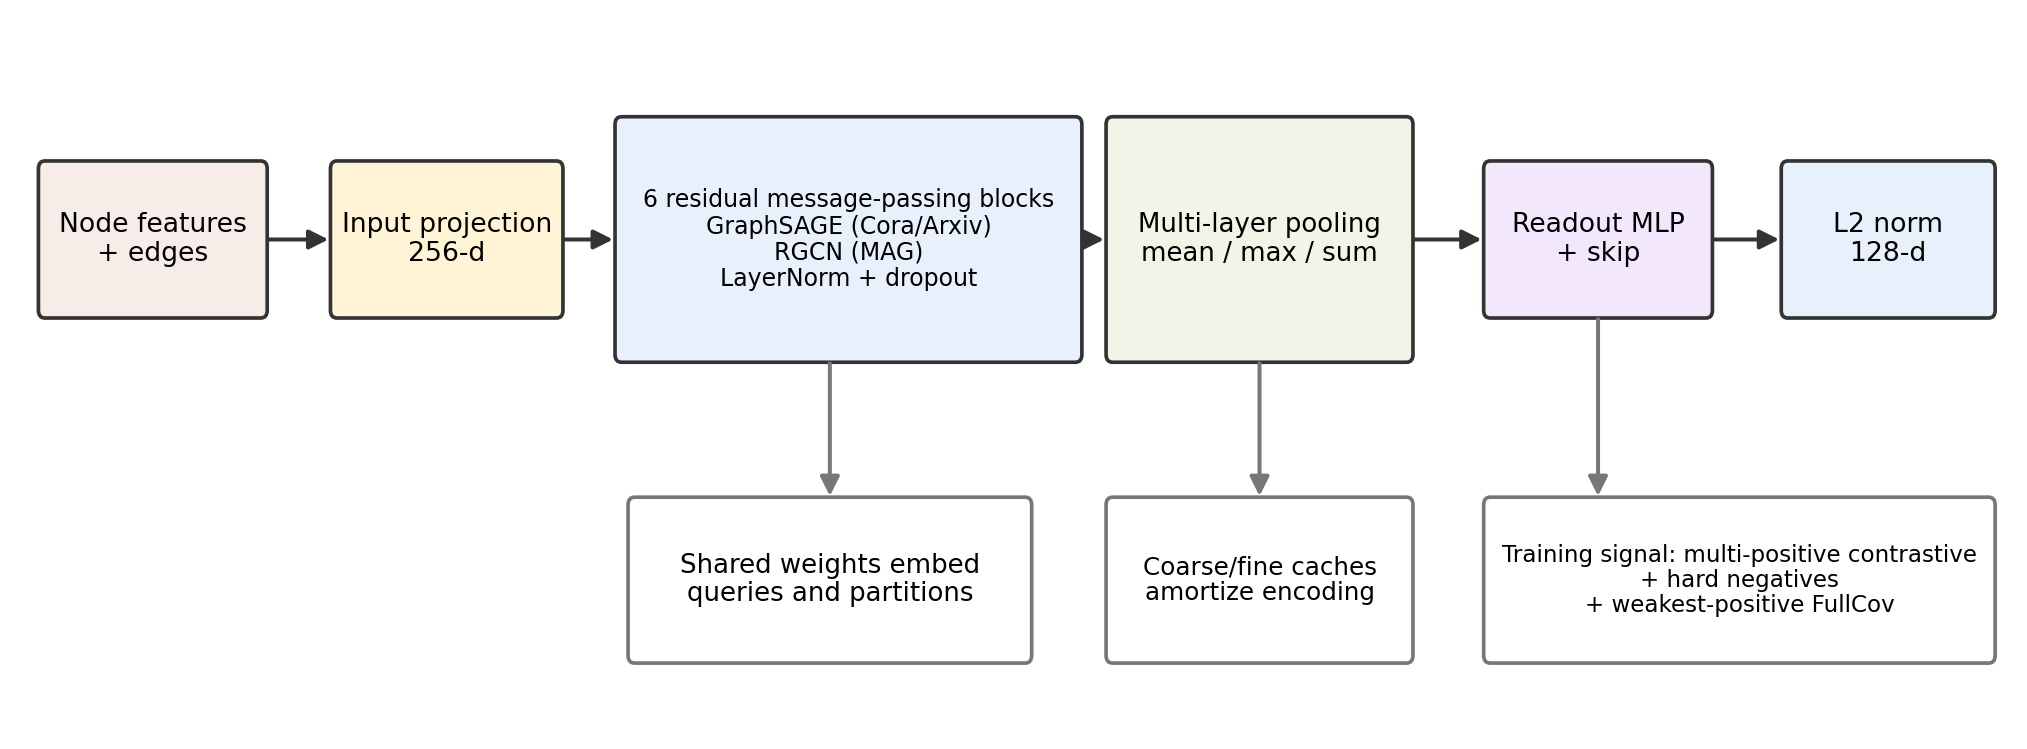
\includegraphics[width=\columnwidth]{fig_encoder_architecture.png}
\caption{\textbf{Shared query/partition encoder.} One network embeds both queries and cached partitions into a common space: six residual GraphSAGE blocks for CoraFull/Arxiv, a relation-aware RGCN for MAG, pooled to an $L_2$-normalized vector and scored by cosine similarity.}
\label{fig:encoder}
\end{figure}

\section{Experimental Protocol}
\label{sec:protocol}

\paragraph{Datasets.}
We evaluate CoraFull~\cite{ref_cora} (small enough for exact timing sanity checks), OGBN-Arxiv~\cite{ref_ogb} ($169{,}343$ nodes, the medium-scale benchmark), and the full heterogeneous OGBN-MAG ($1{,}939{,}743$ nodes across four node types joined by typed relations), which we model relation-aware rather than collapsing to attribute-only structure, stressing both scale and heterogeneity.

\paragraph{Queries and policies.}
All positive families are generated as connected planted subgraphs. The matrix uses two query seeds, sizes $20/50/100$, and $50$ queries per type/size/seed. Positive families are single, multi-fine, K-hop, degree-K-hop, random-walk, and multi-coarse; negatives perturb labels or structure. Retrieval policies are learned Jigsaw, MeanFeat, Mean-RRF (reciprocal-rank fusion of learned and MeanFeat rankings, a configuration of our retriever), TopoFeat, Random, and exhaustive FilterAll; on MAG we additionally run FeatureIndex, a classical label-coverage index. Model selection is protocol-disjoint: the deployed MAG encoder is the checkpoint chosen by validation FullCov on seeds $31415/27182$, while all benchmark queries use seeds $20260607/20260608$, so no benchmark query influenced training, weighting, or checkpoint choice.

\paragraph{Partition and overlap scale.}
On MAG a coarse partition has median $969$ nodes and borders many partitions, but one-hop overlap admits only boundary nodes (median $4{,}252$), not whole neighboring partitions; the loose union bound is never materialized, and pruning leaves much smaller verifier candidates (Section~\ref{sec:results}).

\paragraph{Metrics and hygiene.}
We report FullCov@$K$/recall for retrieval and, for the full path, exact-solve rate, audited no-match accuracy, false positives, timeouts, candidate size, and wall-clock components. Each dataset has $2{,}400$ unique queries ($1{,}800$ positives, $600$ negatives); across three datasets this is $7{,}200$ unique queries. Timings are per-query wall-clock on $8$-vCPU Google Cloud instances with a $30$\,s verifier budget. Encoders, query seeds, hierarchies, and manifests will be released.

\section{Results}
\label{sec:results}

We first isolate the retriever (Section~\ref{sec:fullcov}), then report the end-to-end system across three datasets and the label-selectivity regime (Section~\ref{sec:mainbench}), the headline memory result (Section~\ref{sec:memory}), the encoder-depth diagnostics reviewers of learned components ask for (Section~\ref{sec:depth}), the candidate-shrinkage cascade (Section~\ref{sec:shrinkage}), query families, operator necessity, and soundness.

\subsection{FullCov Training Improves Retrieval}
\label{sec:fullcov}

Table~\ref{tab:loss_ablation} gives the matched-budget Arxiv retrieval result. All rows use the same locked K-hop query seeds and $9{,}000$ optimizer steps. The FullCov objective improves the fixed-budget operating points most relevant to bounded exact verification.

\begin{table}[t]
\centering
\caption{\textbf{Matched Arxiv retrieval objective ablation.} Fixed retrieval budgets on $n{=}400$ locked K-hop queries (200 per query seed); each row averages the validation-selected checkpoint from two independent training replicates.}
\label{tab:loss_ablation}
\small
\setlength{\tabcolsep}{5pt}
\resizebox{\columnwidth}{!}{%
\begin{tabular}{lcccc}
\toprule
\textbf{Objective} & \textbf{FullCov@20} & \textbf{FullCov@50} & \textbf{FullCov@100} & \textbf{Mean worst rank} \\
\midrule
Contrastive control & 21.7\% & 39.0\% & 66.0\% & 74.02 \\
FullCov objective & \textbf{26.0\%} & \textbf{48.8\%} & \textbf{82.0\%} & \textbf{58.97} \\
\midrule
McNemar $p$ & $4.6{\times}10^{-3}$ & $9.8{\times}10^{-6}$ & $4.0{\times}10^{-10}$ & -- \\
\bottomrule
\end{tabular}}
\end{table}

The locked K-hop suite has zero queries impossible at $K{=}20,50,100$; average true coarse footprint is $6.37$ and maximum footprint is $17$. The objective therefore improves ranking by explicitly optimizing the weakest required partition. Because the control and FullCov-aligned models share query seeds and training budget, the gain comes from the objective rather than easier queries or longer optimization. The largest improvement appears at FullCov@100, where the downstream verifier has enough room to benefit from better ordering without searching the whole graph -- exactly the cascade's operating point.

\subsection{Three-Dataset Main Benchmark}
\label{sec:mainbench}

Table~\ref{tab:production_matrix} reports exact planted-match recovery, correct no-match behavior, false positives, solver timeouts, candidate nodes, cascade time, and verifier time. Cascade time sums candidate construction and exact verification and excludes retrieval/ranking.

\begin{table*}[t]
\centering
\caption{\textbf{Main-benchmark metrics.} Pos. uses matched half-partition budgets $K{=}10/100/1000$; FilterAll uses the all-partition ceiling. Neg. is audited no-match accuracy; FP counts negative false positives, while TO counts positive-query solver timeouts (FeatureIndex was run on positives only). Candidate and timing columns use the same endpoint as Pos. Cascade time is candidate construction plus exact verification and excludes retrieval/ranking. Bold marks Jigsaw, the proposed method (not necessarily the per-column maximum); FilterAll is the unbounded exhaustive ceiling and FeatureIndex applies only under near-unique labels.}
\label{tab:production_matrix}
\setlength{\tabcolsep}{6pt}
\small
\begin{tabular}{llrrrrrrr}
\toprule
\textbf{Dataset} & \textbf{Method} & \textbf{Pos. \%} & \textbf{Neg. \%} & \textbf{FP} & \textbf{TO} & \textbf{Cand. nodes} & \textbf{Cascade s} & \textbf{Solver ms} \\
\midrule
CoraFull & Jigsaw & \textbf{94.2} & 100.0 & 0 & 0 & 458 & 0.05 & 11.8 \\
CoraFull & Mean-RRF & 93.8 & 100.0 & 0 & 0 & 485 & 0.05 & 11.8 \\
CoraFull & MeanFeat & 87.7 & 100.0 & 0 & 0 & 1.13K & 0.06 & 10.5 \\
CoraFull & TopoFeat & 31.9 & 100.0 & 0 & 0 & 7.60K & 0.17 & 3.6 \\
CoraFull & Random & 32.7 & 100.0 & 0 & 0 & 7.54K & 0.16 & 3.8 \\
CoraFull & FilterAll$^\ddagger$ & 100.0 & 100.0 & 0 & 0 & 59 & 0.06 & 12.7 \\
\midrule
Arxiv & Jigsaw & \textbf{92.8} & 100.0 & 0 & 0 & 77 & 0.19 & 18.3 \\
Arxiv & Mean-RRF & 94.0 & 100.0 & 0 & 0 & 75 & 0.19 & 18.8 \\
Arxiv & MeanFeat & 89.7 & 100.0 & 0 & 0 & 91 & 0.22 & 18.4 \\
Arxiv & TopoFeat & 33.3 & 100.0 & 0 & 0 & 233 & 0.46 & 6.0 \\
Arxiv & Random & 39.2 & 100.0 & 0 & 0 & 219 & 0.47 & 7.0 \\
Arxiv & FilterAll$^\ddagger$ & 100.0 & 100.0 & 0 & 0 & 57 & 0.35 & 19.1 \\
\midrule
MAG & Jigsaw & \textbf{88.6} & 99.5 & 1 & 25 & 138.1K & 6.97 & 81.9 \\
MAG & Mean-RRF & 85.4 & 99.5 & 1 & 17 & 137.1K & 5.38 & 67.9 \\
MAG & FeatureIndex$^\S$ & 96.7 & -- & -- & 24 & 59.4K & 2.39 & 118.8 \\
MAG & MeanFeat & 64.6 & 99.5 & 1 & 12 & 212.1K & 8.02 & 27.5 \\
MAG & TopoFeat & 37.1 & 99.8 & 1 & 1 & 235.6K & 8.07 & 5.2 \\
MAG & Random & 51.4 & 99.7 & 1 & 9 & 282.1K & 9.54 & 19.9 \\
MAG & FilterAll$^\ddagger$ & 98.4 & 99.3 & 1 & 33 & 443.8K & 5.85 & 288.6 \\
\bottomrule
\end{tabular}
\\[2pt]
\footnotesize $^\ddagger$Exhaustive all-partition ceiling (not a bounded-memory policy). $^\S$Classical label-coverage index; positives only.
\end{table*}

At the half-partition budget (Table~\ref{tab:production_matrix}) Jigsaw solves $94.2/92.8/88.6\%$ on CoraFull/Arxiv/MAG. The $100\%$ CoraFull/Arxiv entries are the exhaustive ceiling, not a retrieval result; Mean-RRF is competitive there, and FeatureIndex is strongest on MAG under near-unique labels. Matched CoraFull/Arxiv costs are measured for every policy: Jigsaw uses mean terminal candidates $458/77$, cascade times $0.05/0.19$\,s, and verifier times $11.8/18.3$\,ms. Size $100$ is harder (CoraFull $89.0\%$ vs. $96.8/96.8\%$ at $20/50$; Arxiv $90.3\%$ vs. $93.8/94.2\%$), driven by CoraFull random-walk ($75.3\%$) and Arxiv multi-coarse ($78.7\%$). On MAG, recovery declines from $93.2\%$ at size $20$ to $90.7\%$ at $50$ and $82.0\%$ at $100$, driven by random-walk, while contained multi-fine remains perfect at every size and multi-coarse remains difficult. Jigsaw sends far fewer candidate nodes than FilterAll ($138$K vs $444$K) at lower verifier time ($82$ vs $289$\,ms), while FilterAll remains the recall ceiling at $98.4\%$.

\paragraph{The scaling break.}
The central systems result is that whole-graph exact matching does not scale: direct CP-based Glasgow solves all $15$ CoraFull K-hop queries but \textbf{0 of 15} on Arxiv and MAG (Table~\ref{tab:scaling_latency}, Figure~\ref{fig:scaling}), whereas the Jigsaw cascade remains feasible by handing the verifier a small candidate. The retriever therefore sits on a recall--cost frontier: FeatureIndex is strongest under near-unique MAG labels, FilterAll is the exhaustive ceiling, and the learned retriever is a useful memory-bounded point, especially once labels coarsen.

\begin{figure}[t]
\centering
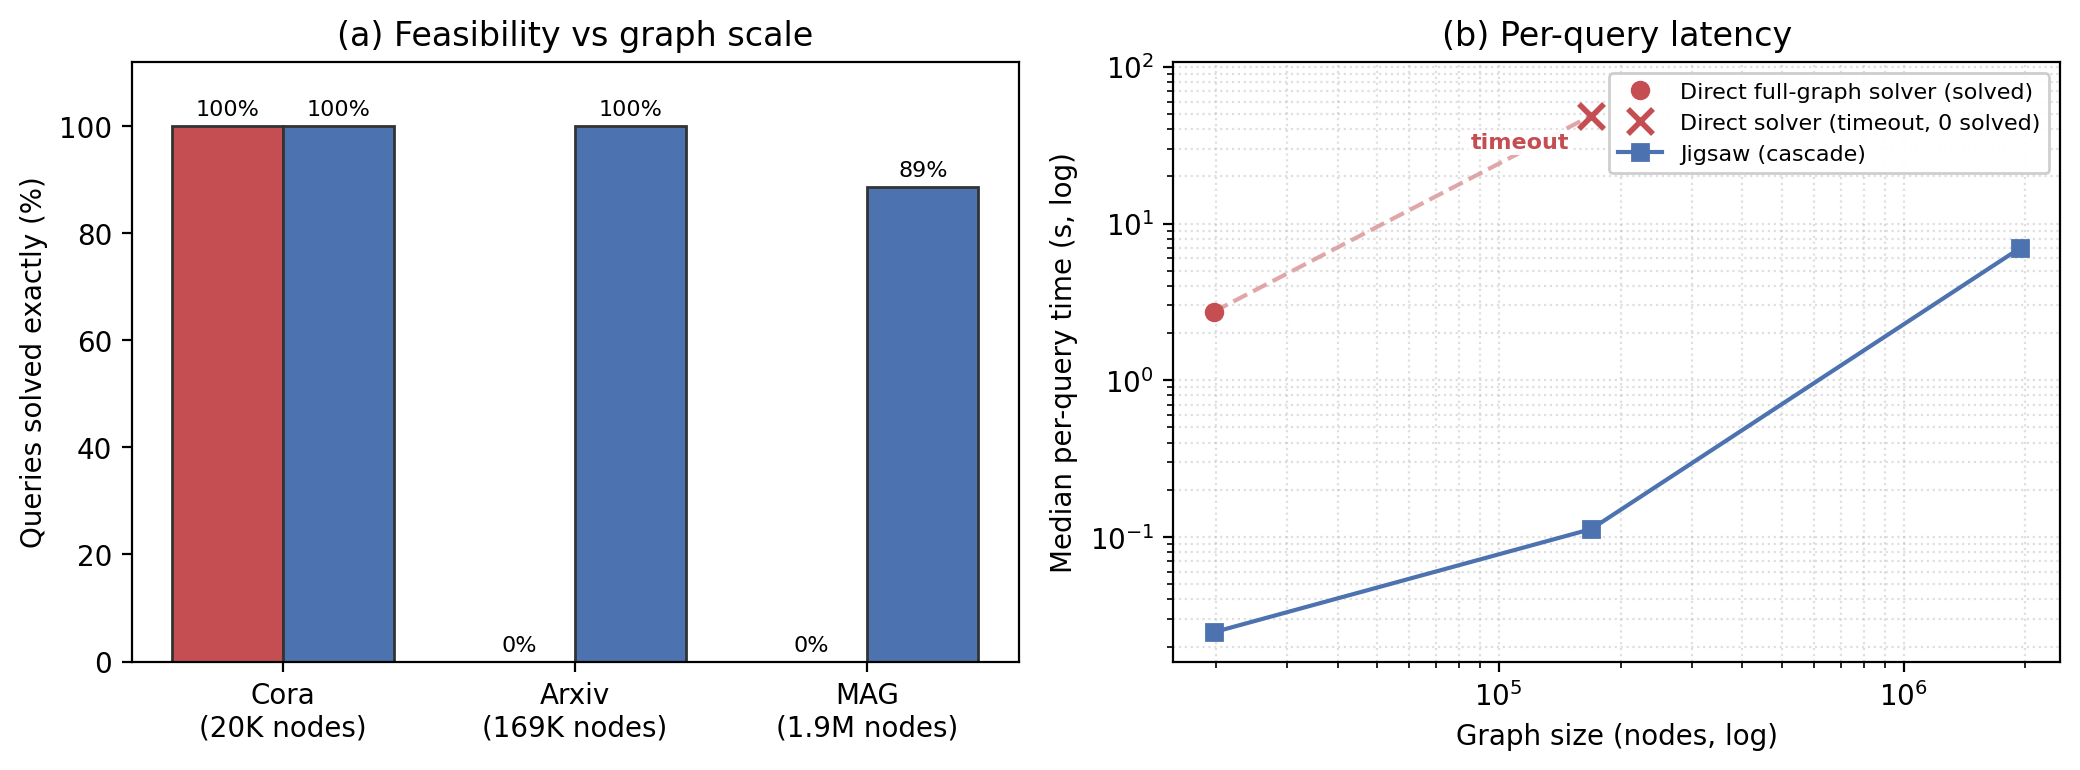
\includegraphics[width=\columnwidth]{fig_scaling_feasibility.png}
\caption{\textbf{Jigsaw makes the exact solver's domain tractable.} Direct full-graph Glasgow solves CoraFull but none of the Arxiv/MAG K-hop samples; Jigsaw stays feasible by verifying only the retrieved-and-pruned candidate.}
\label{fig:scaling}
\end{figure}

\begin{table}[t]
\centering
\caption{\textbf{Scaling and latency: direct full-graph solver vs.\ Jigsaw cascade.} CoraFull/Arxiv use the same 15 K-hop queries; Jigsaw is evaluated at matched half-partition budgets ($K{=}10/100$). The MAG direct cell is its 15-query timeout control; $^\ast$the MAG Jigsaw cell is the 1,800-positive main-benchmark mean at $K{=}1{,}000$.}
\label{tab:scaling_latency}
\small
\resizebox{\columnwidth}{!}{%
\begin{tabular}{l r c r c r r}
\toprule
 & & \multicolumn{2}{c}{Direct full-graph solver} & \multicolumn{2}{c}{Jigsaw cascade} & Cand.\ \\
\cmidrule(lr){3-4}\cmidrule(lr){5-6}
Dataset & Nodes & Solved & Med.\ time & Solved & Med.\ time & nodes \\
\midrule
CoraFull  & 19.8K & 15/15 & $2.74$\,s & 15/15 & $\mathbf{0.03}$\,s & 50 \\
Arxiv & 169K  & \textbf{0/15}$^\dagger$ & ${\approx}49$\,s & 15/15 & $\mathbf{0.11}$\,s & 50 \\
MAG   & 1.9M  & \textbf{0/15} & timeout & 88.6\% & $6.97$\,s$^\ast$ & -- \\
\bottomrule
\end{tabular}}
\end{table}

\paragraph{Label-selectivity crossover.}
Near-unique md5 labels favor exact-label methods: a classical label-coverage index (\textbf{FeatureIndex}, in the GraphGrep~\cite{ref_graphgrep}/gIndex~\cite{ref_gindex} tradition) is the strongest bounded retriever here ($96.7\%$; median worst-true-partition rank $104$ of $2{,}000$) versus the learned GNN ($88.6\%$; rank ${\sim}900$). At coarse $39$-class labels this ranking order \emph{inverts}: the learned model has better worst-true-partition ranks in each family, while complete solve runs are statistically tied (FeatureIndex $63.4\%$; learned variants $63$--$64\%$). This isolates the regime in which learning contributes: as labels stop localizing, the GNN supplies the better partition ranking. The crossover generalizes on CoraFull and Arxiv, where the winner flips with an offline label-selectivity statistic (median partitions/label $1$ at feature labels versus $12$/$124.5$ at class labels), so Jigsaw selects its bounded retriever by label regime (Table~\ref{tab:selectivity_xd}). Jigsaw is therefore \emph{retriever-agnostic}: it routes to a classical index under near-unique labels and to the learned ranker when labels cease to localize.

\begin{table}[t]
\centering
\caption{Cross-dataset label-selectivity crossover: overall median worst-true-partition rank (lower is better; retrieval-only, $n{=}540$ per dataset). Near-unique feature labels favor the classical index; realistic class labels favor the learned retriever.}
\label{tab:selectivity_xd}
\small
\resizebox{\columnwidth}{!}{%
\begin{tabular}{lcccc}
\toprule
 & \multicolumn{2}{c}{FeatureIndex} & Learned & Parts/label \\
\cmidrule(lr){2-3}
Dataset (parts) & feature & class & (any) & feat / class \\
\midrule
CoraFull ($20$)   & 2 & 7   & 5  & $1$ / $12$ \\
Arxiv ($200$) & 4 & 104 & 44 & $1$ / $124.5$ \\
\bottomrule
\end{tabular}}
\end{table}

\paragraph{Statistical significance.}
Table~\ref{tab:significance} reports bootstrap confidence intervals and paired exact-McNemar tests for MAG positives. Jigsaw significantly beats every learned/feature retriever except FilterAll, the exhaustive ceiling. These are component comparisons; the system contribution is exact matching without whole-graph residence and with fewer candidates than FilterAll.

\begin{table}[t]
\centering
\caption{\textbf{MAG solve-rate significance.} Bootstrap 95\% CI over $n{=}1800$ positive queries, and paired exact-McNemar of Jigsaw vs each policy (wins = queries Jigsaw solves and the other does not). The header solve rate and CI are the deployed encoder ($88.6\%$, $1{,}595/1{,}800$); in the paired column Mean-RRF is compared against that deployed run, while MeanFeat/Random/Topo/FilterAll are compared against the encoder-independent Jigsaw run ($86.0\%$, $1{,}548/1{,}800$).}
\label{tab:significance}
\small
\setlength{\tabcolsep}{6pt}
\resizebox{\columnwidth}{!}{%
\begin{tabular}{lccc}
\toprule
\textbf{Method} & \textbf{Solve \%} & \textbf{95\% CI} & \textbf{vs Jigsaw (W/L, $p$)} \\
\midrule
Jigsaw    & 88.6 & [87.1, 90.0] & -- \\
Mean-RRF  & 85.4 & [83.7, 87.0] & 92 / 35, \ $p{=}4.4{\times}10^{-7}$ \\
MeanFeat  & 64.6 & [62.3, 66.8] & 437 / 51, \ $p{<}10^{-76}$ \\
Random    & 51.4 & [49.1, 53.8] & 689 / 67, \ $p{<}10^{-130}$ \\
Topo      & 37.1 & [34.9, 39.5] & 912 / 32, \ $p{<}10^{-224}$ \\
FilterAll & 98.4 & [97.8, 98.9] & 2 / 225, \ $p{=}2.4{\times}10^{-64}$ \\
\bottomrule
\end{tabular}}
\end{table}

\paragraph{Coarse-label stress on resident pipelines.}
The same low-selectivity transition breaks resident exact matchers. With MAG labels coarsened to $32$ deterministic buckets, resident CFL-Match~\cite{ref_cflmatch}/DP-iso~\cite{ref_daf}/GQL~\cite{ref_graphql} complete $12/27$ executions ($8/9$ at size $20$; $2/9$ at each of sizes $50$ and $100$; random-walk $3/9$), with candidate tables reaching $2.4$M entries and $15$ calls hitting the $120$\,s limit. Under near-unique labels the same matchers complete $27/27$: a resident exact solver dominates when selective labels collapse its candidate tables, while under weak labels whole-graph candidate construction is what fails, and Jigsaw's bounded candidate supplies the systems advantage.

\subsection{Memory-Bounded Serving}
\label{sec:memory}

The headline systems benefit is memory. The cascade streams the graph in a two-pass sweep (nodes, then edges) behind an LRU partition cache, so peak resident memory is bounded by the cache rather than by $|G|$. On a $54$-query MAG grid (6 families $\times$ 3 sizes $\times$ 3 queries) the conservative primary serve peaks at \textbf{2.4}\,GB versus \textbf{10.2}\,GB for whole-graph residence ($4.2\times$ smaller), while recovering $46/54$ matches; an optimized cache sweep lowers the eight-partition point to $1.9$\,GB ($5.4\times$). Memory becomes a tunable resource: as the cache grows from $8$ to $256$ partitions, MAG p50 latency falls $5.9{\to}4.8$\,s (below the $8.4$\,s cold load) while the mean holds $17.9{\to}17.6$\,s because of a hard-query I/O tail (Figure~\ref{fig:memory_latency}c). Cold-load end-to-end latency is competitive with resident classical matchers -- $2.35/3.0/1.2\times$ faster on CoraFull/Arxiv/MAG because Jigsaw avoids the full-graph load -- so bounding residence does not cost latency for cold or one-shot queries. A resident matcher, by contrast, amortizes its one-time load and then answers in ${\sim}1$\,ms, so on long repeated-query streams its steady state is faster; Jigsaw's decisive advantage is memory, not latency. An all-or-nothing resident matcher cannot expose this frontier: it must hold the whole graph or fail, whereas Jigsaw lets the operator pick a memory$\leftrightarrow$latency point.

\begin{figure*}[t]
\centering
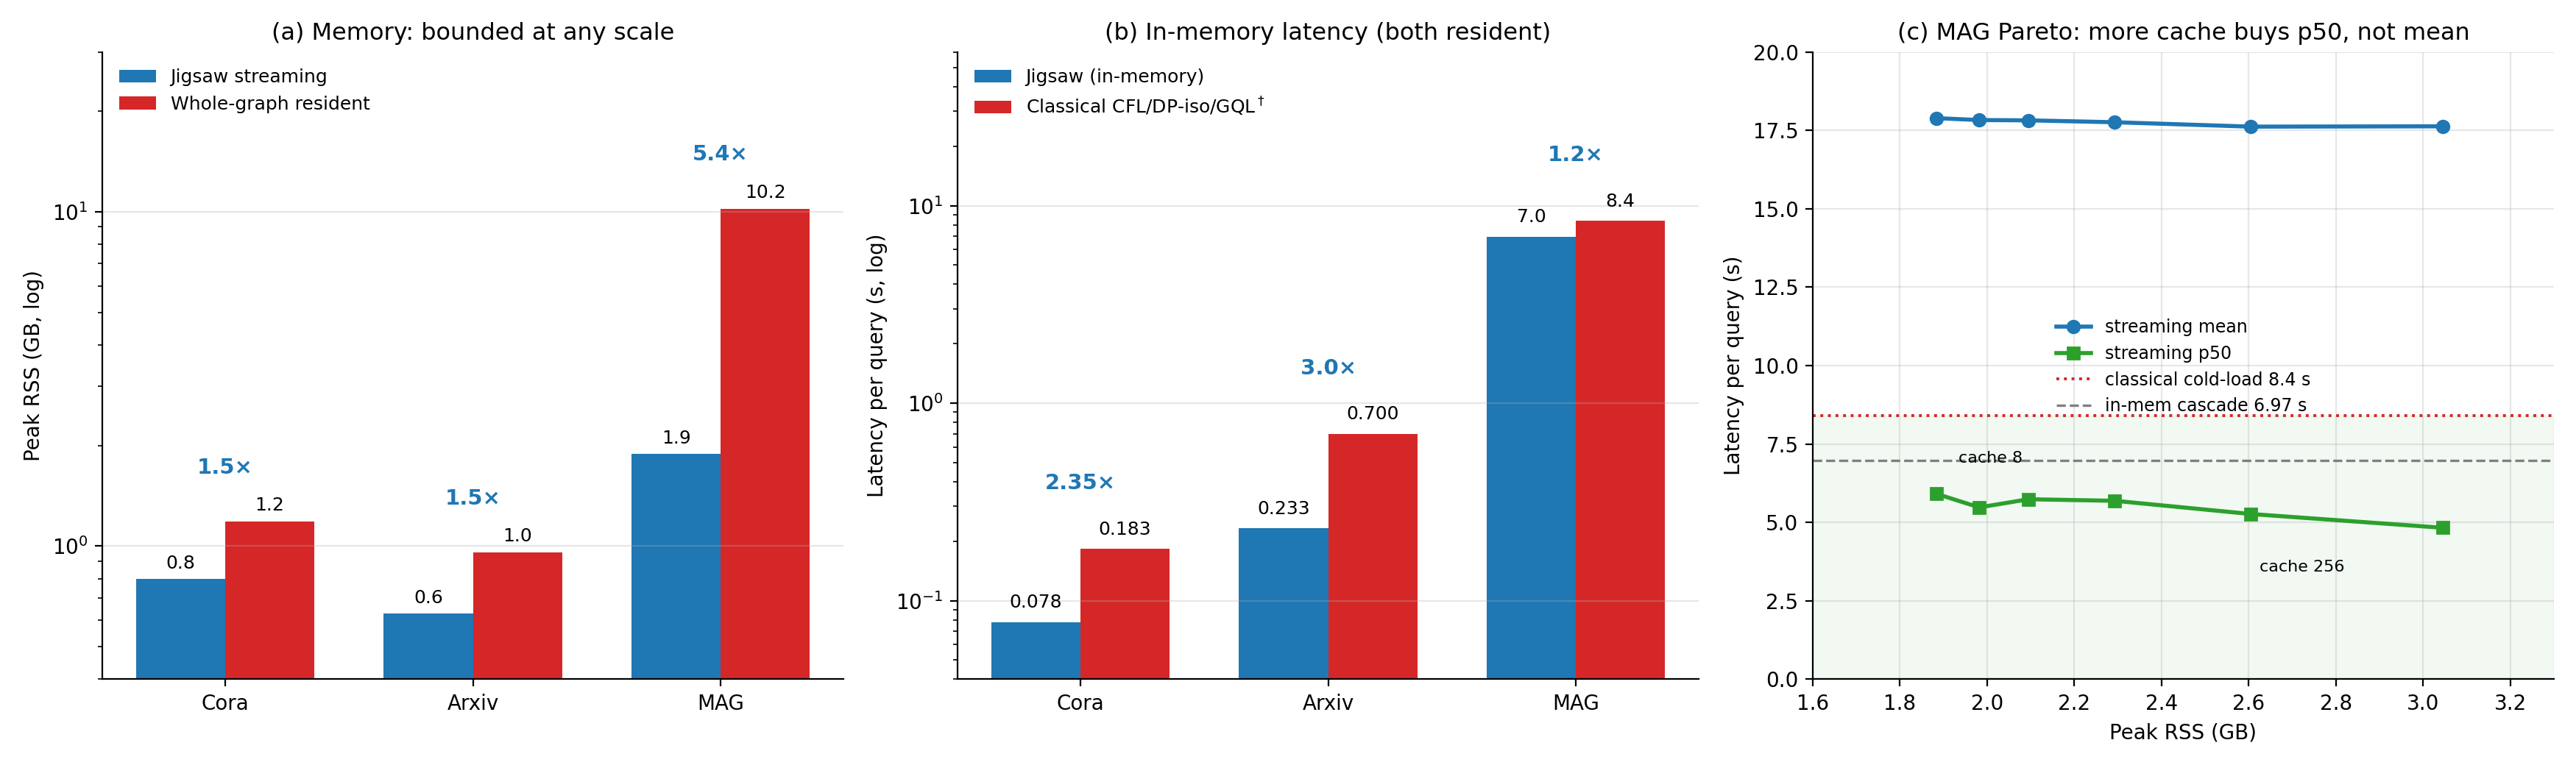
\includegraphics[width=0.92\textwidth]{fig_memory_latency.png}
\caption{\textbf{Memory is the primary benefit; cold-load latency is competitive and the tradeoff is tunable.} \textbf{(a)} The conservative streaming serve is $4.2\times$ smaller on MAG ($2.4$ vs $10.2$\,GB); the optimized cache sweep lowers its eight-partition point to $1.9$\,GB ($5.4\times$). \textbf{(b)} Cold-load latency, Jigsaw vs.\ classical CFL/DP-iso/GQL: $2.35/3.0/1.2\times$ faster on CoraFull/Arxiv/MAG ($^\dagger$MAG resident enumeration is ${\sim}1$\,ms after loading). \textbf{(c)} MAG memory$\leftrightarrow$latency frontier as the cache grows ($8{\to}256$): more memory buys down p50 ($5.9{\to}4.8$\,s) while the mean stays ${\approx}17.6$--$17.9$\,s because of a hard-query I/O tail.}
\label{fig:memory_latency}
\end{figure*}

\subsection{Encoder Depth, Oversmoothing, and Residual Necessity}
\label{sec:depth}

Because Jigsaw depends on a six-layer message-passing encoder, a natural concern is oversmoothing: whether depth collapses node and partition representations. We probe the \emph{deployed} weights (no retrain) and measure, at every layer, node-level mean absolute deviation (MAD $=1-$ mean off-diagonal cosine; $\to 0$ is collapse) and the retrieval-relevant quantity -- effective rank and mean pairwise distance of the mean-pooled \emph{partition} summaries FAISS actually discriminates (Table~\ref{tab:oversmoothing}, Figure~\ref{fig:oversmoothing}).

\begin{table}[t]
\centering
\caption{\textbf{Depth diagnostics on deployed encoders (no retrain).} Partition-summary effective rank and mean pairwise distance from input to layer 6 (higher is better; these are what retrieval discriminates), and the layer-6 node cosine with residual connections disabled ($\to 1$ is textbook collapse). No dataset oversmooths; on GraphSAGE the residual is the anti-collapse mechanism, while the MAG RGCN is robust without it.}
\label{tab:oversmoothing}
\small
\resizebox{\columnwidth}{!}{%
\begin{tabular}{lcccc}
\toprule
 & \multicolumn{2}{c}{Part.\ rank} & \multicolumn{1}{c}{Part.\ dist} & Resid-off \\
\cmidrule(lr){2-3}
Dataset (enc.) & input & L6 & input$\to$L6 & L6 node cos \\
\midrule
CoraFull (SAGE)  & 15.2 & 14.8 & $0.054{\to}0.112$ & 0.965 (collapse) \\
Arxiv (SAGE) & 65.0 & 87.5 & $0.026{\to}0.163$ & 0.951 (collapse) \\
MAG (RGCN)   & 74.5 & 118.9 & $0.062{\to}0.088$ & 0.586 (robust) \\
\bottomrule
\end{tabular}}
\end{table}

\begin{figure}[t]
\centering
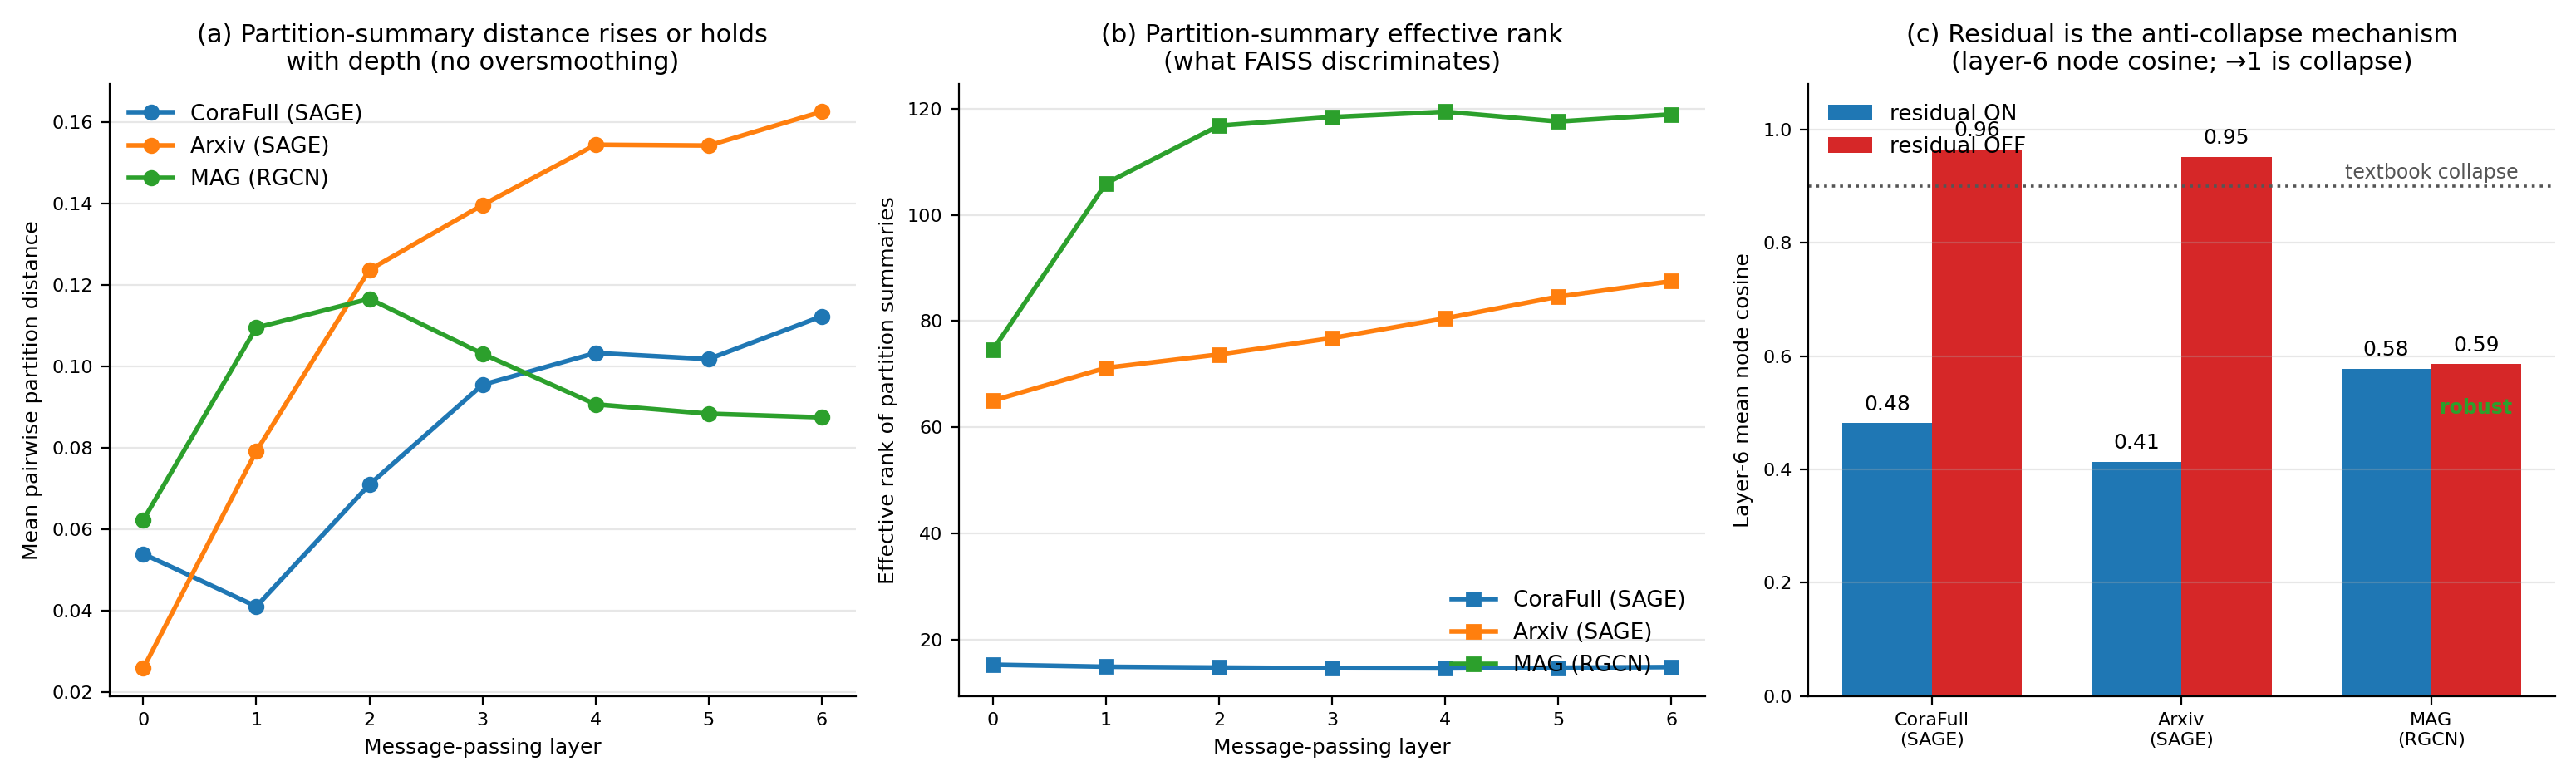
\includegraphics[width=\columnwidth]{fig_oversmoothing.png}
\caption{\textbf{The six-layer encoder does not oversmooth.} Per-layer partition-summary discriminability (the quantity retrieval uses) on the deployed weights: it is preserved on CoraFull, rises with depth on Arxiv and MAG, and only collapses when residual connections are disabled on the GraphSAGE encoders -- isolating the residual as the anti-collapse mechanism.}
\label{fig:oversmoothing}
\end{figure}

Three findings result. \textbf{(1) No oversmoothing at six layers on any dataset.} Partition summaries stay fully discriminable and in fact separate \emph{more} with depth: CoraFull partition distance rises $0.054{\to}0.112$, and MAG partition rank rises $74.5{\to}118.9$ with distance $0.062{\to}0.088$. \textbf{(2) On Arxiv, depth actively helps} -- every metric improves monotonically (node MAD $0.15{\to}0.59$, partition distance $0.026{\to}0.163$, $+240\%$), so six layers are justified rather than harmful. \textbf{(3) Residual connections are the mechanism} on the GraphSAGE encoders: disabling them collapses CoraFull and Arxiv to the textbook regime (layer-6 node cosine $0.965$/$0.951$), whereas the MAG RGCN's per-relation weighting already keeps nodes apart (residual-off cosine $0.586$, no collapse). We therefore keep residual $+$ LayerNorm everywhere for exactly the reason the GraphSAGE case demonstrates. Together with the FullCov objective ablation (Table~\ref{tab:loss_ablation}), this shows the learned component is a well-posed, depth-justified localizer, not a fragile black box.

\subsection{Candidate-Shrinkage Cascade and Boundary Overlap}
\label{sec:shrinkage}

A natural objection is that one-hop overlap might expand to most of the graph. We test the per-query cascade
\[
\text{full graph}\to\text{overlap}\to\text{signature}\to\text{label-prune}\to\text{components}
\]
on $14{,}400$ positive method/model-query evaluation records over the $1{,}800$-query MAG positive grid. Three facts emerge.

\textbf{(1) Overlap is broad, but ranking still removes most of the graph.} The median selected-overlap union is $59\%$ of MAG for Jigsaw, yet after identical pruning the candidate is a median $84.5$K nodes versus $544$K for FilterAll, a $6.4\times$ median reduction (this per-query cascade diagnostic uses the generic-mix encoder over $14{,}400$ records and reports medians; the deployed-encoder \emph{means} are $138$K vs $444$K in Table~\ref{tab:production_matrix}).

\textbf{(2) Pruning is coverage-lossless.} Recall loss occurs at retrieval/overlap, not attribute pruning:

\begin{proposition}[Lossless pruning]
\label{prop:lossless}
Let the pruning token $\sigma(\cdot)$ be a node attribute the matching semantics preserve, i.e.\ any valid embedding $\phi$ of $Q$ into $G$ satisfies $\sigma(\phi(q))=\sigma(q)$ for every query node $q$ (vertex-labelled matching, $\sigma$ derived from node type and feature labels). Prune $G_C$ to $G_C'=\{v\in G_C : \sigma(v)\in \sigma(V_Q)\}$. Then for any embedding $\phi$ with $\phi(V_Q)\subseteq G_C$, we have $\phi(V_Q)\subseteq G_C'$; pruning preserves node coverage and $\mathrm{FullCov}$ is unchanged.
\end{proposition}
\emph{Proof.} For $q\in V_Q$, $\sigma(\phi(q))=\sigma(q)\in\sigma(V_Q)$, so $\phi(q)$ meets the keep condition and is retained. Thus every matched node survives.\hfill$\square$

The cascade signatures and exact-label filters are pure functions of each node's stored attribute vector---node type, hashed feature bits, and (on MAG) quantized per-relation-degree \emph{features} carried verbatim in the query payload, never the query's structural degree recomputed on $Q$---so they are preserved under embedding and the proposition applies. Empirically, planted-match survival after overlap equals survival after pruning for every policy (Jigsaw $87\%$ both), so the solve ceiling is set by whether the retrieved-plus-overlapped region contains the match. \textbf{(3) Candidate construction dominates latency:} mean build is $3.4$\,s for Jigsaw and $5.5$\,s for FilterAll versus $0.25$\,s of solving.

\paragraph{Boundary overlap is an essential recall operator.}
Removing boundary overlap cuts solve rate from $88.9\%$ to $44.4\%$ on MAG and from $94.4\%$ to $86.1\%$ on Arxiv. Its benefit is strongest for compact local structure: boundary expansion recovers missed true partitions for $94\%$ of K-hop queries but $62\%$ of random-walk queries, whose matches more often extend into the interior of an unselected partition. With coverage-lossless pruning, this locates the remaining errors before verification, when retrieval plus boundary overlap does not cover the match.

\subsection{Query Families and Operator Necessity}
\label{sec:family}

\begin{table*}[t]
\centering
\caption{\textbf{Jigsaw query-family breakdown.} Positive columns report exact-solve rate; negative columns report correct no-match rate. All datasets use the connected-positive protocol at the matched half-partition budget ($K{=}10/100/1000$); MAG rows use the deployed encoder (overall $88.6\%$).}
\label{tab:jigsaw_family}
\setlength{\tabcolsep}{6pt}
\small
\begin{tabular}{lrrrrrrrr}
\toprule
\textbf{Dataset} & \textbf{Single} & \textbf{K-hop} & \textbf{Deg-K} & \textbf{Walk} & \textbf{Multi-fine} & \textbf{Multi-coarse} & \textbf{Neg-label} & \textbf{Neg-struct} \\
\midrule
CoraFull & 100.0 & 98.3 & 97.3 & 75.3 & 100.0 & 94.3 & 100.0 & 100.0 \\
Arxiv & 100.0 & 97.3 & 98.3 & 82.3 & 100.0 & 78.7 & 100.0 & 100.0 \\
MAG & 98.7 & 93.3 & 92.7 & 71.0 & 100.0 & 76.0 & 100.0 & 99.0 \\
\bottomrule
\end{tabular}
\end{table*}

The family view (Table~\ref{tab:jigsaw_family}) explains the aggregate rates: single and multi-fine saturate, local K-hop families remain high, and random-walk/multi-coarse are hardest across datasets. Random walks are the main stress test; FilterAll solves them at $96.0\%$, and $96.6\%$ of Jigsaw's random-walk misses occur before solving, locating the opportunity in retrieval and overlap coverage rather than in Glasgow. The held-out deployed encoder lifts random-walk $60.0\%{\to}71.0\%$ and multi-coarse $71.7\%{\to}76.0\%$ over a baseline encoder, showing that learning improves the families in which spatial coverage matters most. Cumulative solved-by-budget curves rise monotonically to $94.2/92.8/88.6$; on MAG the solve rate rises from $37.6\%$ at small budgets to $88.6\%$ at $K{=}1000$, confirming that candidate coverage, not verifier soundness, controls the budget frontier.

\paragraph{What the operator ablations establish.}
The cascade needs multiple operators. At matched budgets, removing overlap lowers solve rate from $88.9$ to $44.4\%$ (MAG) and $94.4$ to $86.1\%$ (Arxiv); removing signatures leaves Arxiv solve rate unchanged but expands mean pruned candidates ${\sim}37\times$ ($76{\to}2{,}815$); removing exact-label pruning and component decomposition drops MAG to $52.8\%$ and $63.9\%$ respectively. Diagnostic variants are kept separate from the canonical validation-selected matrix.

\subsection{Negative Queries and Soundness}
\label{sec:soundness}

Jigsaw never accepts from the neural model alone; Glasgow is the only accepting step. Audited no-match accuracy is $100.0\%$ for CoraFull/Arxiv and $99.3$--$99.8\%$ across MAG policies, with at most one false positive per method; the remaining errors are timeout/unknown outcomes. The rare false positives are benchmark-level, not verifier hallucinations: a returned mapping is a true isomorphism inside the candidate, but a perturbed ``negative'' may still match elsewhere. The reported metric is audited no-match accuracy under this synthetic protocol; global non-existence would require exhaustive full-graph certification, which Jigsaw does not claim.

\section{Related Work}
\label{sec:related}

\paragraph{Exact matchers and in-memory systems.}
Subgraph isomorphism is NP-complete~\cite{ref_garey}. Backtracking matchers from Ullmann~\cite{ref_ullmann} and VF2/VF3~\cite{ref_vf2,ref_vf3} through RI~\cite{ref_ri}, LAD~\cite{ref_lad}, TurboISO~\cite{ref_turboiso}, CFL-Match~\cite{ref_cflmatch}, DP-iso~\cite{ref_daf}, GraphQL~\cite{ref_graphql}, and the more recent VEQ~\cite{ref_veq}, RapidMatch~\cite{ref_rapidmatch}, and CECI~\cite{ref_ceci} improve ordering, pruning, and candidate indexing, and constraint programming yields the strong Glasgow solver~\cite{ref_glasgow} we adopt as the accepting authority. In-depth studies~\cite{ref_survey,ref_survey2024} show these systems are competitive but assume the data graph and its candidate domains are memory-resident -- exactly the assumption that fails at million-node scale and that Jigsaw removes. Worst-case-optimal joins~\cite{ref_wcoj} and GPU matchers~\cite{ref_gsi} attack the join cost rather than residence.

\paragraph{Scale, low memory, and distribution.}
Trinity~\cite{ref_trinity} matches on billion-node graphs with a distributed memory cloud; DualSim~\cite{ref_dualsim} enumerates on a single machine by paging from disk; low-memory dataflows~\cite{ref_lowmem} and G-thinker~\cite{ref_gthinker} shard or stream the whole graph across a cluster. These stream or distribute \emph{the entire graph}; Jigsaw instead pays a one-time partition/index cost and bounds residence by learned relevance, exposing a complementary single-machine memory frontier.

\paragraph{Learned matching and indexing.}
Most neural approaches predict matches or similarity and let the network decide acceptance: NeuroMatch~\cite{ref_neuromatch}, GLSearch~\cite{ref_glsearch}, subgraph counting~\cite{ref_nsic}, SimGNN~\cite{ref_simgnn}, GMN~\cite{ref_gmn}, partition-based hierarchical matching~\cite{ref_psimgnn}, and the ISONET line~\cite{ref_isonet,ref_isonetpp,ref_neuraldesign,ref_neugn}; these typically target smaller or contained queries and trade exactness for a learned score. A second group keeps exactness and uses learning only to prune: GNN-PE~\cite{ref_gnnpe} builds path-dominance embeddings that filter candidates with no false dismissals and then verify exactly, at path granularity and on graphs larger than MAG, and is the closest system to ours. Jigsaw shares that filter-then-verify discipline -- the GNN chooses \emph{where} to verify and Glasgow alone accepts, so exactness is independent of model quality -- but differs in three ways: it retrieves at partition/region granularity rather than per path, it targets \emph{memory-bounded} serving with a tunable memory--latency frontier that GNN-PE and the resident matchers do not expose, and it trades a global no-false-dismissal guarantee for a budget-controlled completeness dial. We run the public GNN-PE release as a transfer diagnostic (Appendix~\ref{app:gnnpe}); a matched-scale head-to-head is future work. Classical structure indices GraphGrep~\cite{ref_graphgrep} and gIndex~\cite{ref_gindex} inspire our FeatureIndex baseline, which we show wins precisely when labels are near-unique. Jigsaw builds on standard components -- GraphSAGE~\cite{ref_graphsage}/RGCN~\cite{ref_rgcn} encoders, METIS partitioning~\cite{ref_metis}, FAISS retrieval~\cite{ref_faiss}, contrastive learning~\cite{ref_cpc}, CVaR~\cite{ref_cvar}, and reciprocal-rank fusion~\cite{ref_rrf} -- and composes them into a retrieval-constrained exact matcher.

\section{Discussion and Limitations}
\label{sec:limits}

Jigsaw is an exact-verification system with a learned search boundary. Retrieval coverage controls completeness while Glasgow preserves sound acceptance inside every candidate; FullCov makes that boundary measurable and trainable. The design targets static attributed graphs and repeated query workloads where partitioning, embeddings, and FAISS indexes amortize; a classical index leads under near-unique labels and learned retrieval becomes the better localizer as labels coarsen, which is why Jigsaw ships both behind an offline selectivity router.

\paragraph{Scope and non-goals.}
We compare against feature/structure index rankers, no-retrieval Glasgow, exhaustive FilterAll, uninformed retrievers, and scalable CFL-Match/DP-iso/GQL controls; these locate Jigsaw's advantage in bounded residence and low-selectivity candidate construction. We do not yet benchmark the most recent in-memory matchers (VEQ, RapidMatch, CECI); like the resident controls we do run, they assume whole-graph residence, so a matched head-to-head at million-node scale is the natural next comparison rather than a threat to the residence argument. Jigsaw does \emph{not} certify global non-existence -- a bounded no-match is not a proof no match exists in $G$ -- and the current benchmark uses planted connected subgraphs on static, single-topology citation graphs, so multi-topology and dynamic-graph generalization remain open. The walk family is the standing recall bottleneck, and the inference-time probes locate its residual errors in representation-level footprint coverage, giving a concrete next learning target. Out-of-core and distributed matchers remain complementary: combining Jigsaw's learned residence bound with sharded verification is promising future work.

\section{Conclusion}
\label{sec:conclusion}

Jigsaw turns learned graph retrieval into an execution mechanism for exact search: the model predicts which regions deserve memory and verification, while Glasgow remains the sole accepting authority. On full MAG this changes the tested operating point from $0/15$ direct solves on the K-hop control to $88.6\%$ exact recovery over $1{,}800$ planted positives, while streaming at $2.4$\,GB instead of $10.2$\,GB for whole-graph residence. FullCov aligns learning with the decisive failure event -- missing even one required partition -- while boundary overlap and coverage-lossless pruning make the verifier usable under bounded memory. Under near-unique labels a resident classical index dominates; under weak labels whole-graph candidate construction fails and Jigsaw's bounded candidate supplies the systems advantage, so Jigsaw is retriever-agnostic by construction. The result is exact subgraph verification made usable on million-node graphs without replacing exactness by a neural guess.

\section*{Acknowledgments}
Generative AI tools assisted with implementation, experiment orchestration, data-validation scripts, and manuscript language editing. The author reviewed and verified all AI-assisted code, analyses, numerical claims, and text, and takes full responsibility for the final work.

\appendix

\section{Encoder and Training Details}
\label{app:encoder}

Beyond the architecture of Section~\ref{sec:encoder} (Figure~\ref{fig:encoder}), the readout is an MLP plus a skip projection before $L_2$ normalization. The message-passing block is GraphSAGE~\cite{ref_graphsage} on CoraFull/Arxiv -- a matched objective ablation finds it at least as strong as GIN~\cite{ref_gin} at the budgets the cascade uses -- and a relation-aware six-layer RGCN~\cite{ref_rgcn} on MAG (per-relation bases over $2R$ symmetrized relations); non-paper MAG nodes, which lack features, receive node-type one-hot and per-relation-degree features. Training combines three signals: paired fine/coarse InfoNCE, hard negatives, and the FullCov coverage term; positive partitions are live re-encoded so coverage gradients update required positives rather than a stale bank. The MAG checkpoint is selected by validation FullCov (seeds $31415/27182$), disjoint from the benchmark seeds. Queries are inductive with respect to an indexed target and need no fine-tuning; a new target pays a one-time METIS hierarchy, partition-embedding, and FAISS build (Table~\ref{tab:deployment_costs}).

\begin{table}[t]
\centering
\caption{\textbf{Representative deployment costs.} Hierarchy loading and combined embedding-plus-index construction are measured setup runs; training is a one-time dataset cost; rank time is query encoding plus FAISS search and excludes candidate construction.}
\label{tab:deployment_costs}
\small
\setlength{\tabcolsep}{5pt}
\resizebox{\columnwidth}{!}{%
\begin{tabular}{lrrrr}
\toprule
Target & Hier.\ load & Embed + index & Enc.\ training & Rank/query \\
\midrule
Arxiv (200 coarse) & 3.5\,s & 1.9\,s & 2--3\,h (9,000 steps) & 5.1\,ms \\
MAG (2,000 coarse) & 110.9\,s & 13.7\,s & ${\sim}3$\,h (5,000 steps) & 21.9\,ms \\
\bottomrule
\end{tabular}}
\end{table}

\section{GNN-PE Public-Release Diagnostic}
\label{app:gnnpe}

Beyond the direct-solver control (Table~\ref{tab:scaling_latency}, $0/15$ on Arxiv/MAG), we ran the public GNN-PE~\cite{ref_gnnpe} release. On CoraFull the released pipeline passes its self-test but, after class-label export and build repairs, recovers $7/24$ planted positives at edit distance $e{=}4$ ($0/6$ at size $100$). The release exposes an inference path but no supervised training recipe for this protocol, so the number measures public-release transfer, not a retrained reproduction; we report it as a transparency control rather than a head-to-head result.

\section{Operator-Necessity Ablation}
\label{app:design}

Table~\ref{tab:design_ablation} gives the per-operator breakdown summarized in Section~\ref{sec:family}. The equal-budget comparison removes the full-budget confound. On MAG, removing one-hop overlap halves solve rate ($88.9{\to}44.4\%$) while signatures are inert; on Arxiv, signatures are the main candidate-control mechanism (mean pruned domain expands ${\sim}37\times$, $76{\to}2{,}815$, when removed) and overlap has a smaller but real effect ($94.4{\to}86.1\%$). Exact-label pruning and component decomposition remain important on MAG ($88.9{\to}52.8\%$ and $88.9{\to}63.9\%$).

\begin{table}[t]
\centering
\caption{\textbf{Operator-necessity ablation at matched half-partition budgets.} The shared diagnostic has 48 queries per dataset; solve/candidate statistics use its 36 planted positives (MAG at $K{=}1{,}000/2{,}000$, Arxiv at $K{=}100/200$).}
\label{tab:design_ablation}
\small
\setlength{\tabcolsep}{6pt}
\resizebox{\columnwidth}{!}{%
\begin{tabular}{lrrrr}
\toprule
 & \multicolumn{2}{c}{\textbf{OGBN-MAG}} & \multicolumn{2}{c}{\textbf{OGBN-Arxiv}} \\
\cmidrule(lr){2-3}\cmidrule(lr){4-5}
\textbf{Variant} & \textbf{Solve \%} & \textbf{Cand.} & \textbf{Solve \%} & \textbf{Cand.} \\
\midrule
Full Jigsaw    & 88.9          & 150.6K & 94.4 & 76 \\
No overlap     & \textbf{44.4} & 152.5K & \textbf{86.1} & 88 \\
No signature   & 88.9          & 150.7K & 94.4 & \textbf{2{,}815} \\
No components  & 63.9          & 143.0K & 94.4 & 76 \\
No exact-label & 52.8          & 223.6K & 94.4 & 244 \\
\bottomrule
\end{tabular}}
\end{table}

\section{Partition and Overlap Scale}
\label{app:partitions}

For a selected coarse partition, the overlap operator adds only boundary nodes from partitions sharing an edge with it, not the bordering partitions in full. On MAG a median partition ($969$ nodes) borders $948$ of $2{,}000$ coarse partitions but admits only ${\approx}4{,}252$ boundary nodes, so the expanded region is ${\approx}5{,}228$ nodes -- a $5.4\times$ expansion, not the ${\approx}921$K a whole-neighbor union would give. That loose bound is a reachability figure the operator never realizes; reporting it as ``the overlap'' overstates MAG breadth by more than $170\times$. Candidate breadth arises only when the cascade unions boundary overlap across hundreds of retrieved partitions, and because many boundary nodes are shared the union saturates between $59\%$ (Jigsaw) and $83\%$ (uninformed policies) of MAG at the largest budgets.

\section{Retrieval-Remedy Foreclosure and Within-MAG Selectivity}
\label{app:probes}

A natural question is whether a cheaper inference-time change to retrieval would close the spatial-family gap without retraining. It does not. On MAG, subquery multi-vector MaxSim, finer partition parents, one- and two-hop fine-level overlap, dual-granularity late interaction, and coarse diffusion all leave FullCov@$1000$ within ${\approx}2$ points of the single-vector baseline on the k-hop/degree-k-hop/random-walk families (Table~\ref{tab:probes_log}); the best gain is ${\approx}{+}2.3$ (coarse diffusion) and a coarse neighbor-stitch expansion \emph{reduces} coverage by $8$--$13$ points. The cause is density: the partition graph is high-degree at every granularity (median coarse degree $948$; mean fine degree $568$ of $10{,}000$), so neighborhood-following broadens the candidate rather than tracing the query footprint. This directs further improvement toward coverage-aware representation learning rather than inference-time patching.

\begin{table}[t]
\centering
\caption{Inference-time remedies on the same 1,800-query MAG positive workload: FullCov@$1000$ (\%). Each displayed spatial family has $n{=}300$ queries.}
\label{tab:probes_log}
\small
\resizebox{\columnwidth}{!}{%
\begin{tabular}{lrrr}
\toprule
Method & k-hop & degree-k-hop & random-walk \\
\midrule
Single-vector (current)           & 14.7 & 17.3 & 9.0 \\
Subquery MaxSim (query-only)      & 14.3 & 17.7 & 8.0 \\
Finer partition parent            & 12.7 & 16.7 & 8.3 \\
Fine-level overlap (1-hop)        & 13.3 & 17.3 & 10.0 \\
Fine-level overlap (2-hop)        & 13.3 & 18.3 & 9.3 \\
Dual-granularity late interaction & 12.7 & 16.0 & 8.7 \\
Coarse diffusion                  & 17.0 & 19.7 & 10.3 \\
\bottomrule
\end{tabular}}
\end{table}

The selectivity crossover of Section~\ref{sec:mainbench} also appears \emph{within} MAG. Holding the $1.9$M-node target fixed and shrinking the md5 codebook from $10^{6}$ to $10^{2}$ labels drives the median partitions spanned by a label from $1$ to $1{,}938$; the learned ranker never uses this codebook, so its coverage is flat, while FeatureIndex begins at the ceiling and falls monotonically, crossing below the learned ranker family by family (Table~\ref{tab:mag_selectivity_sweep}). This reproduces the cross-dataset inversion on a single deployed target, confirming the learned advantage is a low-selectivity phenomenon rather than a dataset artifact.

\begin{table}[t]
\centering
\caption{\textbf{Within-MAG label-selectivity sweep} (FullCov@$1000$, feature-driven families, $n{=}300$ each). As the md5 codebook shrinks, partitions/label grows and FeatureIndex coverage falls below the \emph{label-independent} learned ranker (bottom row, flat by construction).}
\label{tab:mag_selectivity_sweep}
\small
\setlength{\tabcolsep}{6pt}
\resizebox{\columnwidth}{!}{%
\begin{tabular}{lrrr}
\toprule
Median parts/label & Single & Multi-fine & Multi-coarse \\
\midrule
$1$ (near-unique)   & 100.0 & 100.0 & 99.0 \\
$7$                 & 100.0 & 100.0 & 99.0 \\
$74$                & 100.0 & 100.0 & 94.0 \\
$636$               & 100.0 & 100.0 & 59.3 \\
$1{,}938$           & 76.0  & 78.7  & 14.0 \\
\midrule
Learned (flat)      & \textbf{99.3} & \textbf{99.7} & \textbf{65.0} \\
\bottomrule
\end{tabular}}
\end{table}

\begin{thebibliography}{45}

\bibitem[McCreesh et al.(2020)]{ref_glasgow}
McCreesh, C., Prosser, P., Trimble, J.: The Glasgow Subgraph Solver: Using Constraint Programming to Tackle Hard Subgraph Isomorphism Problem Variants. In: CP 2020, LNCS, vol. 12333, pp. 316--333. Springer (2020)

\bibitem[Xu et al.(2019)]{ref_gin}
Xu, K., Hu, W., Leskovec, J., Jegelka, S.: How Powerful are Graph Neural Networks? In: ICLR (2019)

\bibitem[Hamilton et al.(2017)]{ref_graphsage}
Hamilton, W.L., Ying, R., Leskovec, J.: Inductive Representation Learning on Large Graphs. In: NeurIPS, pp. 1024--1034 (2017)

\bibitem[Schlichtkrull et al.(2018)]{ref_rgcn}
Schlichtkrull, M., Kipf, T.N., Bloem, P., van den Berg, R., Titov, I., Welling, M.: Modeling Relational Data with Graph Convolutional Networks. In: ESWC, pp. 593--607 (2018)

\bibitem[Cordella et al.(2004)]{ref_vf2}
Cordella, L.P., Foggia, P., Sansone, C., Vento, M.: A (Sub)Graph Isomorphism Algorithm for Matching Large Graphs. IEEE TPAMI \textbf{26}(10), 1367--1372 (2004)

\bibitem[Johnson et al.(2021)]{ref_faiss}
Johnson, J., Douze, M., J\'egou, H.: Billion-Scale Similarity Search with GPUs. IEEE Trans. Big Data \textbf{7}(2), 535--547 (2021)

\bibitem[Karypis and Kumar(1998)]{ref_metis}
Karypis, G., Kumar, V.: A Fast and High Quality Multilevel Scheme for Partitioning Irregular Graphs. SIAM J. Sci. Comput. \textbf{20}(1), 359--392 (1998)

\bibitem[Hu et al.(2020)]{ref_ogb}
Hu, W., et al.: Open Graph Benchmark: Datasets for Machine Learning on Graphs. In: NeurIPS (2020)

\bibitem[Garey and Johnson(1979)]{ref_garey}
Garey, M.R., Johnson, D.S.: Computers and Intractability: A Guide to the Theory of NP-Completeness. W.H. Freeman (1979)

\bibitem[Ullmann(1976)]{ref_ullmann}
Ullmann, J.R.: An Algorithm for Subgraph Isomorphism. J. ACM \textbf{23}(1), 31--42 (1976)

\bibitem[Bonnici et al.(2013)]{ref_ri}
Bonnici, V., Giugno, R., Pulvirenti, A., Shasha, D., Ferro, A.: A Subgraph Isomorphism Algorithm and Its Application to Biochemical Data. BMC Bioinformatics \textbf{14}(Suppl 7), S13 (2013)

\bibitem[Solnon(2010)]{ref_lad}
Solnon, C.: AllDifferent-Based Filtering for Subgraph Isomorphism. Artificial Intelligence \textbf{174}(12--13), 850--864 (2010)

\bibitem[Bojchevski and G\"unnemann(2018)]{ref_cora}
Bojchevski, A., G\"unnemann, S.: Deep Gaussian Embedding of Graphs: Unsupervised Inductive Learning via Ranking. In: ICLR (2018)

\bibitem[Ying et al.(2020)]{ref_neuromatch}
Ying, R., et al.: Neural Subgraph Matching. arXiv:2007.03092 (2020)

\bibitem[Ye et al.(2024)]{ref_gnnpe}
Ye, Y., Lian, X., Chen, M.: Efficient Exact Subgraph Matching via GNN-based Path Dominance Embedding. Proc. VLDB Endow. \textbf{17}(7), 1628--1641 (2024)

\bibitem[Liu et al.(2021)]{ref_glsearch}
Liu, Y., et al.: GLSearch: Maximum Common Subgraph Detection via Learning to Search. In: ICML (2021)

\bibitem[Liu et al.(2020)]{ref_nsic}
Liu, X., Pan, H., He, M., Song, Y., Jiang, X., Shang, L.: Neural Subgraph Isomorphism Counting. In: KDD (2020)

\bibitem[Han et al.(2013)]{ref_turboiso}
Han, W.S., Lee, J., Lee, J.H.: TurboISO: Towards Ultrafast and Robust Subgraph Isomorphism Search in Large Graph Databases. In: SIGMOD, pp. 337--348 (2013)

\bibitem[Bi et al.(2016)]{ref_cflmatch}
Bi, F., Chang, L., Lin, X., Qin, L., Zhang, W.: Efficient Subgraph Matching by Postponing Cartesian Products. In: SIGMOD, pp. 1199--1214 (2016)

\bibitem[Han et al.(2019)]{ref_daf}
Han, M., Kim, H., Gu, G., Park, K., Han, W.S.: Efficient Subgraph Matching: Harmonizing Dynamic Programming, Adaptive Matching Order, and Failing Set Together. In: SIGMOD, pp. 1429--1446 (2019)

\bibitem[He and Singh(2008)]{ref_graphql}
He, H., Singh, A.K.: Graphs-at-a-Time: Query Language and Access Methods for Graph Databases. In: SIGMOD, pp. 405--418 (2008)

\bibitem[Kim et al.(2021)]{ref_veq}
Kim, H., Choi, Y., Park, K., Lin, X., Hong, S.H., Han, W.S.: Versatile Equivalences: Speeding up Subgraph Query Processing and Subgraph Matching. In: SIGMOD, pp. 925--937 (2021)

\bibitem[Sun et al.(2020)]{ref_rapidmatch}
Sun, S., Sun, X., Che, Y., Luo, Q., He, B.: RapidMatch: A Holistic Approach to Subgraph Query Processing. Proc. VLDB Endow. \textbf{14}(2), 176--188 (2020)

\bibitem[Bhattarai et al.(2019)]{ref_ceci}
Bhattarai, B., Liu, H., Huang, H.H.: CECI: Compact Embedding Cluster Index for Scalable Subgraph Matching. In: SIGMOD, pp. 1447--1462 (2019)

\bibitem[Carletti et al.(2018)]{ref_vf3}
Carletti, V., Foggia, P., Saggese, A., Vento, M.: Challenging the Time Complexity of Exact Subgraph Isomorphism for Huge and Dense Graphs with VF3. IEEE Trans. Pattern Anal. Mach. Intell. \textbf{40}(4), 804--818 (2018)

\bibitem[Zeng et al.(2020)]{ref_gsi}
Zeng, L., Zou, L., \"{O}zsu, M.T., Hu, L., Zhang, F.: GSI: GPU-friendly Subgraph Isomorphism. In: ICDE, pp. 1249--1260 (2020)

\bibitem[Sun and Luo(2020)]{ref_survey}
Sun, S., Luo, Q.: In-Memory Subgraph Matching: An In-depth Study. In: SIGMOD, pp. 1083--1098 (2020)

\bibitem[Zhang et al.(2024)]{ref_survey2024}
Zhang, Z., Lu, Y., Zheng, W., Lin, X.: A Comprehensive Survey and Experimental Study of Subgraph Matching: Trends, Unbiasedness, and Interaction. Proc. ACM Manag. Data \textbf{2}(1), Article 60 (2024)

\bibitem[Mhedhbi and Salihoglu(2019)]{ref_wcoj}
Mhedhbi, A., Salihoglu, S.: Optimizing Subgraph Queries by Combining Binary and Worst-Case Optimal Joins. Proc. VLDB Endow. \textbf{12}(11), 1692--1704 (2019)

\bibitem[Ammar et al.(2018)]{ref_lowmem}
Ammar, K., McSherry, F., Salihoglu, S., Joglekar, M.: Distributed Evaluation of Subgraph Queries Using Worst-Case Optimal Low-Memory Dataflows. Proc. VLDB Endow. \textbf{11}(6), 691--704 (2018)

\bibitem[Kim et al.(2016)]{ref_dualsim}
Kim, H., Lee, J., Bhowmick, S.S., Han, W.-S., Lee, J., Ko, S., Jarrah, M.H.A.: DUALSIM: Parallel Subgraph Enumeration in a Massive Graph on a Single Machine. In: SIGMOD, pp. 1231--1245 (2016)

\bibitem[Sun et al.(2012)]{ref_trinity}
Sun, Z., Wang, H., Wang, H., Shao, B., Li, J.: Efficient Subgraph Matching on Billion Node Graphs. Proc. VLDB Endow. \textbf{5}(9), 788--799 (2012)

\bibitem[Yan et al.(2020)]{ref_gthinker}
Yan, D., Guo, G., Chowdhury, M.M.R., \"{O}zsu, M.T., Ku, W.-S., Lui, J.C.S.: G-thinker: A Distributed Framework for Finding Qualified Subgraphs in a Big Graph with Load Balancing. In: ICDE (2020)

\bibitem[Bai et al.(2019)]{ref_simgnn}
Bai, Y., Ding, H., Bian, S., Chen, T., Sun, Y., Wang, W.: SimGNN: A Neural Network Approach to Fast Graph Similarity Computation. In: WSDM, pp. 384--392 (2019)

\bibitem[Li et al.(2019)]{ref_gmn}
Li, Y., Gu, C., Dullien, T., Vinyals, O., Kohli, P.: Graph Matching Networks for Learning the Similarity of Graph Structured Objects. In: ICML, PMLR \textbf{97}, 3835--3845 (2019)

\bibitem[Xu et al.(2021)]{ref_psimgnn}
Xu, H., Duan, Z., Wang, Y., Feng, J., Chen, R., Zhang, Q., Xu, Z.: Graph Partitioning and Graph Neural Network Based Hierarchical Graph Matching for Graph Similarity Computation. Neurocomputing \textbf{439}, 348--362 (2021)

\bibitem[Roy et al.(2022)]{ref_isonet}
Roy, I., Velugoti, V.S.B.R., Chakrabarti, S., De, A.: Interpretable Neural Subgraph Matching for Graph Retrieval. In: AAAI \textbf{36}(7), 8115--8123 (2022)

\bibitem[Ramachandran et al.(2024)]{ref_isonetpp}
Ramachandran, A., Raj, V., Roy, I., Chakrabarti, S., De, A.: Iteratively Refined Early Interaction Alignment for Subgraph Matching Based Graph Retrieval. In: NeurIPS \textbf{37} (2024)

\bibitem[Raj et al.(2025)]{ref_neuraldesign}
Raj, V., Roy, I., Ramachandran, A., Chakrabarti, S., De, A.: Charting the Design Space of Neural Graph Representations for Subgraph Matching. In: ICLR (2025)

\bibitem[Ying et al.(2026)]{ref_neugn}
Ying, Y., Dai, Y., Li, W., et al.: Neural Graph Navigation for Intelligent Subgraph Matching. In: AAAI \textbf{40}(19), 16181--16189 (2026)

\bibitem[Shasha et al.(2002)]{ref_graphgrep}
Shasha, D., Wang, J.T.L., Giugno, R.: Algorithmics and Applications of Tree and Graph Searching. In: PODS, pp. 39--52 (2002)

\bibitem[Yan et al.(2004)]{ref_gindex}
Yan, X., Yu, P.S., Han, J.: Graph Indexing: A Frequent Structure-based Approach. In: SIGMOD, pp. 335--346 (2004)

\bibitem[van den Oord et al.(2018)]{ref_cpc}
van den Oord, A., Li, Y., Vinyals, O.: Representation Learning with Contrastive Predictive Coding. arXiv:1807.03748 (2018)

\bibitem[Rockafellar and Uryasev(2000)]{ref_cvar}
Rockafellar, R.T., Uryasev, S.: Optimization of Conditional Value-at-Risk. Journal of Risk \textbf{2}(3), 21--41 (2000)

\bibitem[Cormack et al.(2009)]{ref_rrf}
Cormack, G.V., Clarke, C.L.A., Buettcher, S.: Reciprocal Rank Fusion Outperforms Condorcet and Individual Rank Learning Methods. In: SIGIR, pp. 758--759 (2009)

\end{thebibliography}

\end{document}
